\documentclass{ximera}


\graphicspath{
  {./}
  {ximeraTutorial/}
  {basicPhilosophy/}
}

\newcommand{\mooculus}{\textsf{\textbf{MOOC}\textnormal{\textsf{ULUS}}}}

\usepackage{tkz-euclide}\usepackage{tikz}
\usepackage{tikz-cd}
\usetikzlibrary{arrows}
\tikzset{>=stealth,commutative diagrams/.cd,
  arrow style=tikz,diagrams={>=stealth}} %% cool arrow head
\tikzset{shorten <>/.style={ shorten >=#1, shorten <=#1 } } %% allows shorter vectors

\usetikzlibrary{backgrounds} %% for boxes around graphs
\usetikzlibrary{shapes,positioning}  %% Clouds and stars
\usetikzlibrary{matrix} %% for matrix
\usepgfplotslibrary{polar} %% for polar plots
\usepgfplotslibrary{fillbetween} %% to shade area between curves in TikZ
\usetkzobj{all}
\usepackage[makeroom]{cancel} %% for strike outs
%\usepackage{mathtools} %% for pretty underbrace % Breaks Ximera
%\usepackage{multicol}
\usepackage{pgffor} %% required for integral for loops



%% http://tex.stackexchange.com/questions/66490/drawing-a-tikz-arc-specifying-the-center
%% Draws beach ball
\tikzset{pics/carc/.style args={#1:#2:#3}{code={\draw[pic actions] (#1:#3) arc(#1:#2:#3);}}}



\usepackage{array}
\setlength{\extrarowheight}{+.1cm}
\newdimen\digitwidth
\settowidth\digitwidth{9}
\def\divrule#1#2{
\noalign{\moveright#1\digitwidth
\vbox{\hrule width#2\digitwidth}}}






\DeclareMathOperator{\arccot}{arccot}
\DeclareMathOperator{\arcsec}{arcsec}
\DeclareMathOperator{\arccsc}{arccsc}

















%%This is to help with formatting on future title pages.
\newenvironment{sectionOutcomes}{}{}


\author{Lee Wayand}

\begin{document}
\begin{exercise}  





Below is the graph of $y=A(r)$.  

\begin{image}
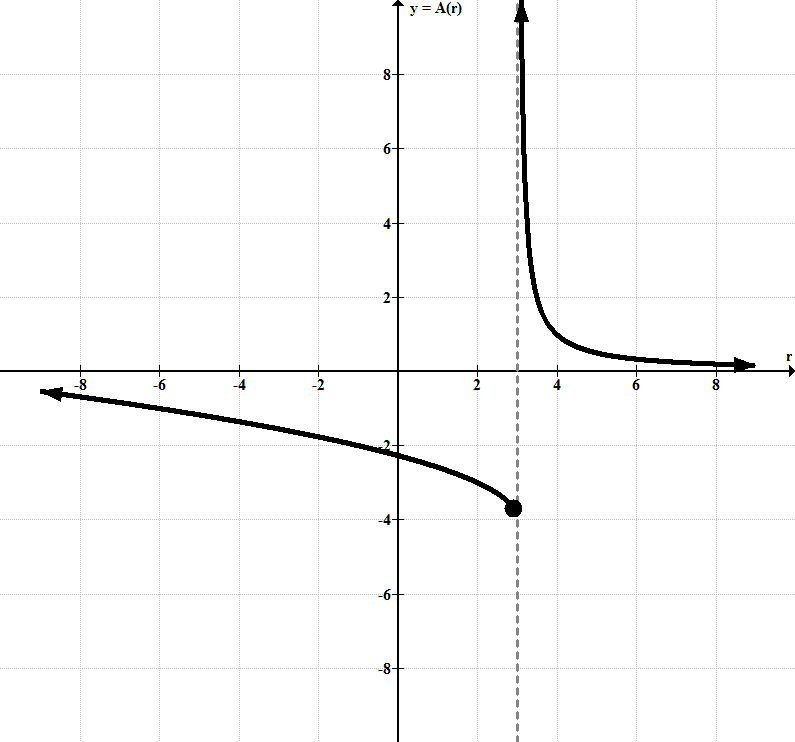
\includegraphics{../../pics/func_graphs/f19.png}
\end{image}









\begin{question} 


What is the domain of $A$?\\


\begin{multipleChoice}
\choice {$[-9, 9]$}
\choice {$(-\infty, 3) \cup (3, \infty)$}
\choice {$\{ 3 \} \cup (3, \infty)$}
\choice [correct]{$(-\infty, \infty)$}
\end{multipleChoice}

\end{question}






\begin{question} 


What is the range of $A$?\\


\begin{multipleChoice}
\choice {$(-\infty, \infty)$}
\choice {$(-\infty, 3] \cup (3, \infty)$}
\choice {$[-3.8, \infty)$}
\choice [correct]{$[-3.8, 0) \cup (0, \infty)$}
\end{multipleChoice}


\end{question}









\begin{question} 



\[  A(0) = \answer[tolerance=0.25]{-2.2}  \]

\end{question}










\begin{question} 



$A(r)$ is a decreasing function.
\begin{multipleChoice}
\choice {True}
\choice [correct]{False}
\end{multipleChoice}

\end{question}







\begin{question} 



$A(r)$ is a decreasing function on any interval inside the domain.
\begin{multipleChoice}
\choice [correct]{True}
\choice {False}
\end{multipleChoice}

\end{question}






\begin{question} 



The minimum of $A(r)$ is $\answer[tolerance=0.25]{-3.7}$.   \\

The maximum of $A(r)$ is $\answer{DNE}$.
 

\end{question}












\end{exercise}
\end{document}